\documentclass[12pt]{report}
\usepackage[margin=1in]{geometry}
\usepackage{multicol}
\usepackage{caption}
\usepackage{subcaption}
\usepackage{graphicx}
\usepackage{float}
\usepackage{epstopdf}
\usepackage{setspace}
\usepackage{abstract}
%\usepackage{grffile}
\usepackage{pdfpages}
\usepackage{lscape}
\usepackage{authblk}
\usepackage{hyperref}

%Graphics Path
\graphicspath{{./MCINTOSH_Images/}{./WILEY_Images/}{./KIRBY_Images/}{./WESLEY_Images/}{./IANNUCCI_Images/}{./BLUM_Images/}{./REGAN_Images/}}

\usepackage{fancyhdr}
	\pagestyle{fancy}
	\fancyhead[L]{\today}
	\fancyfoot{}
	\fancyhead[C]{OCE 496 Section 2}
	\fancyhead[R]{\thepage}


\title{\vspace{-5mm}
	\fontsize{20pt}{10pt}\selectfont
	Embedded Wireless Sensor Design for Long Term Structural Health Monitoring
}
		
\author[2]{Christopher Bessin}	
\author[1]{Patrick Blum}
\author[1]{Matthew P. Iannucci}
\author[1]{Jordan T. Kirby}
\author[1]{Zachary McIntosh}
\author[2]{Elizabeth L. Paul}
\author[1]{Michael A. Regan}
\author[2]{Justin W. Skenyon}
\author[1]{Charles J. Wesley}
\author[1]{Samuel D. Wiley}

\affil[1]{Finite Element Modelling}
\affil[2]{Instrumentation Development}
\date{\normalsize\vspace{-3mm}\today}



\begin{document}
\maketitle

%Signature Block

\textit{I have read this paper in its entirety and approve it for submission.}
\vspace{1.5cm}

\noindent\begin{tabular}{ll}
\makebox[2.5in]{\hrulefill} & \makebox[2.5in]{\hrulefill}\\
Christopher Bessin & Date\\[4ex]% adds space between the two sets of signatures
\makebox[2.5in]{\hrulefill} & \makebox[2.5in]{\hrulefill}\\
Patrick Blum & Date\\[4ex]
\makebox[2.5in]{\hrulefill} & \makebox[2.5in]{\hrulefill}\\
Matthew P. Iannucci & Date\\[4ex]
\makebox[2.5in]{\hrulefill} & \makebox[2.5in]{\hrulefill}\\
Jordan T. Kirby & Date\\[4ex]
\makebox[2.5in]{\hrulefill} & \makebox[2.5in]{\hrulefill}\\
Zachary McIntosh & Date\\[4ex]
\makebox[2.5in]{\hrulefill} & \makebox[2.5in]{\hrulefill}\\
Elizabeth L. Paul & Date\\[4ex]
\makebox[2.5in]{\hrulefill} & \makebox[2.5in]{\hrulefill}\\
Michael A. Regan & Date\\[4ex]
\makebox[2.5in]{\hrulefill} & \makebox[2.5in]{\hrulefill}\\
Justin W. Skenyon & Date\\[4ex]
\makebox[2.5in]{\hrulefill} & \makebox[2.5in]{\hrulefill}\\
Charles J. Wesley & Date\\[4ex]
\makebox[2.5in]{\hrulefill} & \makebox[2.5in]{\hrulefill}\\
Samuel D. Wiley & Date\\[4ex]
\end{tabular}

%Abstract Here


\begin{abstract}
Structural Health monitoring is the process of evaluating and assessing fatigue of existing infrastructure by continuously monitoring a long term change in
natural frequency vibration. Aging traffic infrastructure is a growing problem across the world as material and construction cost has risen considerably in
recent decades. As replacement becomes more difficult reliable lifetime extension is possible through structural health monitoring. At the completion of
this project a sensory package was designed and partially assembled, A simple finite element model (FEM) of the main span was produces, high precision
GPS units were installed and collected data for two weeks, and preliminary data was collected with the package accelerometers on top of the towers of
the bridge. With development and research damage location, type, and severity may be indicated by interpreting the vibration changes. \\

\end{abstract}


\tableofcontents
\listoffigures
\listoftables

\chapter{Introduction}
\label{ch:Paper_Introduction}
	\section{Objectives}
		\subsection{Phase One}
		\subsection{Phase Two}
	\section{Layout}
		%\chapter*{Layout} 

\indent This report will discuss the planning process of designing a sensor package intended to evaluate vibration on the Claiborne Pell Bridge. As this is a
two-semester project the preliminary assembly of the package was simplified to evaluate vibrations of a 6.8 meter angle beam in phase one. A finite element
model was produced of this angle beam to provide information on the modes of vibration and natural frequency. In the second semester the package was
further developed but not completed. Data was collected from the top of the towers by a prototype package. A FEM was produced of the Claiborne Bridge
and used to evaluate approximate natural frequencies of the bridge and to indicate where the package should be installed for best results. \\

\indent Chapter \ref{ch:FEM} explains the process of the finite element model that was produced for both the angle beam and the Claiborne Bridge. The specific
parameters  used to describe the material are described in detail. To prove that the finite element model was reflecting accurate natural frequencies and
modes of vibration, the model for the angle beam was verified with an analytical solution. \\
\indent Choosing appropriate cooperating instrumentation is critical to producing a sensor package that will accurately monitor vibration frequencies.
Chapter \ref{ch:Instrumentation} of this report will present the instrumentation chosen and why. \\
\indent Three separate data sets were recorded; that of the angle beam, the bridge, and the battery discharge curve. The collection process and processing
details are discussed in Chapter \ref{ch:DataCollection}. \\ 
\indent The verifications and comparisons of the various data sets collected are discussed in Chapter \ref{ch:DataAnalysis} along with other discussion about the data
%This next paragraph is quite weird Elizabeth :P 
\indent As the package was not finished to completion, the future developments that are required to make this package whole are indicated in Chapter \ref{ch:FutureDevelopment}.
There were five systems that were not implemented; wireless communication capabilities, the GPS time synchronization, power independence, and total assymbly. Chapter \ref{ch:FutureDevelopment} describes the measures that need to be taken to complete the sensor package.\\

		
\chapter{Finite Element Model (FEM)}
\label{ch:FEM}
	\chapter{Finite Element Model (FEM)}

\section{Introduction}

\label{sec:examples}

\subsection{Background of the Claiborne Pell Bridge}

The Pell Bridge is 10,3471 in total length and has a main span on 1,601 feet making it the 83rd largest suspension bridge in the world. Traffic from
Aquidneck Island would otherwise have to drive around the bay through Providence if the Newport Bridge did not exist. The original proposal for the
bridge was submitted in 1950 by the designer of the New York City subway system and the Cape Cod Canal, and was approved in 1965. The concrete footings
the support the two towers are supported by 838 driven steel piles. At a water depth of 162 feet the foundation created for the Newport Bridge
involved the deepest pile driving in the world at this time. To accelerate cutting the tops of the piles, a dive tank was sunk that housed the divers
for a weeks at a time. Barges brought prefabricated sections of the bridge to Newport where they were lifted into place; the largest of the sections
weighted more than 400 tons and stood 10 stories high. 90,000 cubic yards of concrete were poured into the 52 piers \cite{RIBTA}\\ 

\subsection{Introduction to FEM}

A finite element model analyzes the physical response of a system to dynamic or static loading. The system is divided into finite elements and material
structural properties are applied. The physical response of the structure to an applied loading is added to the initial configuration of the structure.
Abaqus is a computer software which calculates approximate non linear finite element solutions for displacements, deformation, stresses, forces, etc. .
The state of the model is updated throughout the analysis steps and the effects of the previous step are included in the solution to each iteration
\cite{Abaqus}. The stiffness matrix and friction between elements are considered in its original state and updated after each iteration. \cite{Manoj}\\

\indent To verify the software the analysis of a simple system can be completed analytically and compared with the results of the program. For a simply
supported beams the modal shapes are trivial, however, the modal response for a complex structure, like the Claiborne Pell Bridge, anticipating modal
response is near impossible with analytical solutions. \\
\indent Abaqus provides multiple ways to model a particular structure. When modeling the Newport Bridge it will be necessary to use the physical
properties, such as length and profile, rather than physical properties, such as moment of inertia, to model efficiently. To ensure that Abaqus is
calculating moment of inertia as anticipated, analytical solutions can be compared with the results modal frequencies of the Abaqus model. Abaqus allows
for two different options of modeling, inputting the moment of inertia or imputing the profile of the element and allowing Abaqus to calculate moment
of inertia. \\
\indent Within a model produced in Abaqus, the removal of members allows for the structural integrity of the structure to be evaluated as an incomplete
system. Future construction can be aided by this as the ability to see if a partial structure can support itself. The loss of structural components can
be evaluated if lost as well. If a tower were to be damages by a boat or a hanger were to fail, the repercussion could be evaluated. 

\section{Abaqus FEM Verification}

\subsection{L Beam Analysis}

As Abaqus is solving Euler-Bernoulli beam theory equations and iterating the solution over a system, if the system is simple the analytical solution can be
found by hand. For the modal analysis of the 6.8 meter L beam, the beam was modeled two different ways in Abaqus. This was done to confirm that Abaqus
calculates the mode shapes and associated frequencies properly. The analytical solution was calculated using this Equation:


\ref{eqn:FEM_Anal}\\

\begin{equation}

F_{n}=\frac{1}{2\pi}\biggl[\frac{n \pi}{L} \biggr]^{2}\sqrt{[\frac{EI}{\rho}} , n=1,2,3\dots\infty

\label{eqn:FEM_Anal}

\end{equation}

\noindent The inputs for the analytical calculations and the Abaqus model are displayed in Table (Table 

\ref{tab:FEM_Abaqus_Comp}):\\

\indent The beam was modeled in Abaqus as 6.8 meters long, with the supports 0.35 meters from either end. There is a tri-axial restriction boundary
condition at one end and a vertical restriction boundary condition at the other. For the initial model, an undefined profile was used and the moment of
inertia and cross sectional area were input. In the second model, a preset profile was used and Abaqus calculated the moment of inertia. Thickness and
outer dimension of the beam were input. A comparison of the results of those models are presented in comparison to the analytical calculation as
follows:

(Table \ref{tab:FEM_Abaqus_Comp}):\\

\begin{table}[H]

\begin{center}

\begin{tabular}{|l| p{3.5cm}| p{3cm}| p{3cm}| p{3cm}|}

\hline

\textbf{Mode} & \textbf{Analytical Values} & \textbf{General Profile Abaqus Model Frequency}& 

\textbf{Input Profile Abaqus Model Frequency} \\\hline

1 & 3.1 Hz & 3.1 Hz & 3.1 Hz \\\hline

2 & 12.4 Hz & 12.5 Hz & 12.4 Hz \\\hline

3 & 27.9 Hz & 27.8 Hz & 27.8 Hz \\\hline

4 & 49.6 Hz & 48.8 Hz & 48.6 Hz \\\hline

5 & 77.5 Hz & 74.5 Hz & 74.4 Hz \\\hline

\end{tabular}

\caption{\textit{Comparison between Abaqus models}}

\label{tab:FEM_Abaqus_Comp}

\end{center}

\end{table}

\indent The frequencies of the analytical solution and the Abaqus model are very close. This is very important to the progression of this project as
Abaqus must be trusted to calculate the moment of inertia within the program, translating to correct modal shapes and frequencies. \\
\indent Analysis of an I beam was done as preliminary model verification and can be found in the Appendix ******. Because the corresponding frequencies
for the first 5 modes are more than three orders of magnitude larger than that is expected of the Claiborne Bridge (0.155-0.993Hz vs 17.6-230.1Hz), and
intentions for the beam were to test accelerometer setups to be used on the bridge, analysis was not continued on the I-beam and the L-beam was
introduced. 

\section{Claiborne Pell Bridge Model}

\subsection{Modeling Large Suspension Bridges}
The complexity and variability of large suspension bridges makes both numerical and experimental methodology very difficult and requires many assumptions.
As material and construction technologies advance, so do the length and structural complexity of these structures grow. Monitoring and measuring the
structural integrity of these bridges is very important as fatigue is very difficult to measure and quantify. Of the failure endured by steel
structures, 80-90\% are related to fatigue \cite{Chan}. Fatigue analysis includes evaluating the distribution of stress in structures.\\
\indent Long suspension bridges are very flexible and lightly damped structures that are largely impacted by the dynamic loading of cars, wind, and
environmental factors. Fatigue damage will result in large infrastructure due long-term cyclic loading in a corrosive environment
\cite{Chan,Guo,Li:2003}. As with many bridges that experience extreme season change, the Claiborne Pell Bridge is subject to varying temperature change,
snow loading, and salting in addition to the range of other challenges. 


\subsection{Modeling Process}

The purpose of the analysis of the model in Abaqus is to understand the bridge behavior during static loading. As the physical properties of the bridge
structural elements must be reflected in the model, the method of translating the blueprint in ABAQUS properly is vital to producing accurate results.
The main span of the Claiborne Pell Bridge was modeled in MKS (meter, kilogram, second) units. Each of the 8,233 elements were given the appropriate
dimension and material properties to reflect the beams and cables the Claiborne Pell Bridge. There are five structural components of a suspension
bridge 

which will be discussed in detail:

\begin{enumerate}
\item Main cables
\item Towers that support the cable system
\item Hanger cables
\item Anchor bolts that support the cable system at the ends of the cable
\item Hanger cables that connect the main cable to the deck
\item Girder
\end{enumerate}

\subsubsection{Main Cables and Hanger Cables}

Suspension bridges are the lightest bridges per foot made possible because by the weight bearing abilities of the cables which are made of thousands of
pencil-thin steel wires. Steel that is stretched into wires can withstand more stress. The tension force applied to the bridge girder are transferred to
the main cables through the hangers. The cables are very still and flex very little but need to allow for dynamic loading and vibrations \cite{manoj}.
The hanger and main cables are very complicated to model as they must be modeled with the anticipation that after loaded they will accurately represent
the physical shape and rigidity of the actual cables. It is now routine to measure the actual initial stresses in the hangers and main cables upon
construction to input into Abaqus for Eigenvalue analysis. As initial stress in the hangers and main cable will significantly affect the structural
stiffness matrix, K, it is imperative that this value be accurate. The Eigen values were calculated as follows: 

% FIX EQUATION 

\begin{equation}

( 2 \mu[M] + \mu[C] + [K]){\Phi} = 0

\label{eqn:Euler}

\end{equation}

Where [M] is the mass matrix, [C] is the damping matrix, and [K] is the stress matrix, $\mu$ is the 

eigenvalue, and $\Phi$ is the eigenvector \cite{manoj}. 

\subsubsection{Towers}

Made of steel, the towers are subjected to compressive forces induced by the main cables. They need to be sturdy enough to resist buckling, oscillations,
and flexing. The materials of towers is typically steel but in appropriate environments, concrete enforced steel is chosen. The current speed, price,
appearance, and whether salt water or fresh water is being gaped will depict what material is chosen \cite{manoj}. 


\subsubsection{Anchor Bolts}

Anchor piers bear the weight of the main cables and fix them in place. The anchor piers for the Claiborne Pell Bridge are 40x50x100 feet above the MWL and
weigh approximately 3,950 tons each. The weight of the anchor piers hold the cables in place. 

\subsubsection{Girder}

The function of the girder is to stiffen the roadway and support the road deck which carries traffic. The girder is very stiff and thus inhibits large
variations in the road deck as concentrated loads travel over the bridge.\\ 
\indent It was the unfavorable trapezoidal shape of the girder that lead to the collapse of the Tacoma Bridge. The span to width ratio and shape allowed
wind excite the bridge dramatically. After the collapse of the Tacoma Bridge the girder shapes were made to be more stiff with diagonal supports and
square rather than sharp edged \cite{manoj}. 

\subsection{Limitations of Abaqus Model}

\indent Although finite element analysis has enables engineers and scientists gain an understanding of a structure's behavior and dynamic response, it is
very important to know the limitations of finite element modeling. Abaqus must be used as a research tool and not considered the basis of design
\cite{Abaqus}. When verifying experimental data, a FEM should not be used for analysis as too many variables that can not be measured or controlled. \\
\indent In phase one of this project and indicating a particular profile, the preset profiles that are available do not match identically with the
profiles that were used in experiments. The taper of the flange and the radius of the angle were not taken into account in the profile provided by
Abaqus. As the frequencies resultant for the two different modeling techniques were not considerably different, the error acquired within the
dissimilarity is assumed not to be significant and thus neglected in evaluations. \\
\indent In phase two of this project, many assumptions and simplifications were made to allow for preliminary modeling. The method of modeling for this
semester does not consider mated elements; the entire structure is considered as one highly elastic structure with varying physical properties rather
than many different pieced welded or joined with bolts. This affects how the bridge moves as no friction between parts and no welds are considered. 
\indent Fatigue damage is local failure mode and occurs most often in welded regions and thus the model should include the detailed welded region
connection points. The stress fluctuations are very low so the structure will deform elastically except in the welded regions. Critical locations for
fatigue damage can be identified by global stress estimation. As the properties of the bridge elements \cite{manoj}\\

\chapter{Instrumentation Package}
\label{ch:Instrumentation}
	\section{Introduction}
		\section{Introduction}
The sensor package created this semester is a primitive prototype with
bare functionality with respect to the final product. The final
product sensor package is planned to be an autonomous sensor package
capable of transmitting strain gauge and accelerometer data
wirelessly to a base monitoring station. The package will also
be synced with other sensors monitoring the same structure so the
base station can collect synchronized data from multiple locations
on the structure. \\

The package that has been developed at this stage of the project does
not have some of the important functionality that the final project
is expected to have. Phase 1 prototype has the ability to
collect strain gauge and accelerometer data over a sampling
period at a given sampling rate. The timing of the data
collection was driven by an external clock source. Each sample
is given a timestamp with a GPS device and logged to a file
for manual analysis. At this point in time, multiple packages
were not time synchronized, nor were wireless communications
possible. This current package is quite modular, and has
mulyiple sub-systems, detailed in the following
sections.

	\section{Microprocessor}
		\label{sec:uProcessor}
		\section{Microprocessor}
\label{sec:uProcessor}
\indent At the core of the sensor package is the microprocessor. The
microprocessor served as the data collection and distribution
device. The module received data from the peripheral devices and
either stored the data for further analysis or distributed it in
some manner. However, because of both the project requirements
and the diversity of the sensors, choosing the right
microprocessor meant looking closely at all of the requirements
for operation. These requirements may be seen below. 
\subsection{Necessary Specifications}
\subsubsection{Power Consumption}

\indent Though power was not a focus of this semester, the
microprocessor of choice was to be used through the next semester
as well. This means the module of choice should be low power and
made for embedded applications. 

\subsubsection{Timing Accuracy and Synchronization}

\indent Another important area to consider is the ability to time
synchronize with a central clock. This was also not a concern for
the prototyping stage this semester but the same board will be used
for the coming semester. In some way it must be feasible for the
computer chosen to communicate with a clock source and
synchronize itself. This could mean communicating with an
external GPS module or with a remote NTP server. 
\subsubsection{Sampling Frequency}

The microprocessor must be able to sample data from peripheral sensors at a rate fast enough to avoid aliasing data. Analysis from the Finite Element Modeling team was used to decide on this parameter

\subsubsection{Input Output Capabilities}

In order for the processor to collect and relay data from many
different sensors, there are strict input output needs. To
communicate with the Analog to Digital Converter (ADC), the
computer needs to have an Inter-Integrated Circuit ($I_2C$) bus.
Two Universal Asynchronous Receiver/Transmitter (UART) buses are
needed to communicate with the GPS module and a wireless
transmitter that has not been determined yet.

\subsubsection{Data Logging}

For testing, the ability to store data to a log file instead of
exporting via wireless was desired. This allowed testing of the
prototype without the use of wireless communications. The data
could be collected and simply stored for later analysis. 


\subsubsection{Software Development}

The platform chosen should a reasonably tested development
environment and SDK. The platform chosen should have a compiler
that makes use of popular languages. It should also be clear, if
more than one language may be used, what the advantages and
disadvantages of each approach would be. For instance, compiling
an executable vs executing a python script. 

\subsection{Platform Options}

\subsubsection{Microprocessor Comparison Table}
\begin{table}
\centering
\begin{tabular}{|l| p{3cm} | p{3cm} |}
\hline
\textbf{Microprocessor:} & BeagleBone Black 
%	\begin{figure}
\includegraphics[scale = 0.25]{BeagleBoneBlack_Image.jpg}
%	\end{figure}
& Netburner MOD5270
%	\begin{figure}
\includegraphics[scale = 0.25]{Netburner_MOD5270_Image.jpg}
%	\end{figure}
\\
\hline
\textbf{Clock Rate:}		&1GHz ARM Cortex-A8& 145.7MHz 
Freescale ColdFire 5270 \\
\hline
\textbf{I/O Pins:}		& 65  &46\\
\hline
\textbf{Power Consumption:}&	1.05-2.3 W @ 5V	& 1.65 W @ 3.3V	\\
\hline
\textbf{Data Storage:}	&			microSD		&	microSD	\\
\hline
\textbf{Supported Communications:}&	I$^2$C, SPI, 3 Serial 
Ports		&I$^2$C, QSPI, 3 Serial Ports		\\
\hline
\textbf{Software Development}&Python,C/C$^{++}$&C/C$^{++}$\\
\hline
\end{tabular}
\caption{\textit{Comparison table of two microprocessors that 
were looked into for the embedded sensor package}}
\label{tab:uProcOptions}
\end{table}

\subsubsection{BeagleBone Black}
\label{subsec:BeagleBoneBlack}
\indent The BeagleBone Black is single board computer (SBC) that
runs a Linux operating system (Angstrom). The board is powered by a
TI AM3358 Sitara ARM Cortex-A8 Microprocessor. The core is 32 bit,
and can reach up to 1 GHz clock speeds. The board comes with a
plethora of pins. Included are two $I_2C$ buses, four UART
ports, and over 60 GPIO pins. There are also ground, 3.3V, and
5V pins to drive peripheral devices. \\

\indent The board runs full blown Linux and root access is
available. This means that development is possible with a variety
of languages from C++ to Java-script More importantly, there are
third party API (Application Programming Interface) libraries for
the all of the board's input and output written for both Python
and Java-script Both are high level languages and allow for
efficient code development and quicker testing of hardware
development. 

\subsubsection{Netburner MOD5270}
\label{subsec:MOD5270}
\indent The Netburner MOD5270 is a powerful embedded
micro-controller The drawing feature of this board is the inclusion
of a real time clock and its Real Time Operating System. It brings
predictable multitasking and timing. Furthermore, there is an
on-board SD card slot that can be used for real time data
logging. The processor is a 32-bit Freescale ColdFire 5270
running at 145.7 MHz. The on-board Direct Memory Access (DMA)
timers are optimal for timing the application and
synchronizing data transfers. There are two UARTs and an
$I_2C$ bus to go along with various General Purpose
Input/Output (GPIO) pins, including interrupt enabled pins
for external triggering if necessary. \\

\indent The board has a C++/C cross compiler. The System Development
Knowledge (SDK) is well documented and there are many examples for
various applications. The Netburner does not run a full operation
system. Instead, it runs a Real Time Operating System which
handle multitasking with priority levels and cycling. This is
much preferred to a full operating system for an embedded system
as it makes timing more precise and the processor more
efficient. However, the downside to the low level nature of
the board is the development difficulty. The development is
more difficult and takes more time and precision to
perfect. It is also more difficult to modify than a higher
level program running atop a traditional OS layer as seen
in the BeagleBone Black.

\subsection{Platform Decision}

The BeagleBone Black was the single board computer chosen for the
system. The system clock is fast enough to handle data at a rate of
1 kHz, the maximum sampling rate that was used for data
collection. Also, there are four serial buses, so the board was
able to receive data from the external GPS receiver module.
Importantly, the board allowed for fast development with the
Analog to Digital converter chosen. Development would have
been much slower if a different board had been chosen. The
board was chosen because of its ability to satisfy all of the
requirements for the microprocessor while allowing for
dynamic testing throughout the prototyping stage. 

	\section{Sensors}
		\subsection{Accelerometer}
			\subsection{Accelerometer}
\indent Accelerometers were implemented in this package to determine the frequencies at which the element vibrates at. For lab testing, the desired data was the modal shapes of an L beam. The use of accelerometers for structural health monitoring is becoming common practice in smart bridges such as the new I-35W bridge in Minneapolis where periodic modal studies are performed\cite{Kistler}.

\subsection{Accelerometer Parameters}
\indent When choosing the correct accelerometer to be implemented in the sensor package, the following parameters were deciding factors:
\begin{itemize}
\item Number of Axes
\item Dynamic Range
\item Type of Mount
\item Analog vs Digital Output
\item Bandwidth
\item Power Consumption
\end{itemize}

\subsubsection{Number of Axes}
\indent The number of axes is regarded as how many directions that acceleration may be measured. Typically accelerometers have at least two axis. For the purposes of the sensor package, three axis were needed.
\subsubsection{Dynamic Range}
\indent The main limiting factor for determining the proper accelerometer was the dynamic range (DR).  This refers to the range of accelerations that the sensor is capable of measuring. For a 3g accelerometer, the device can measure accelerations up to $3*9.81m/s^{2})$ or$ 29.43 m/s^{2}$.  The value of the dynamic range is found on its corresponding data sheet.  To determine the appropriate accelerometer, the proper DR had to be determined.  This value is a dependent upon three parameters.  The equation for the dynamic range , Equation \ref{eqn:Acc_Accel} below, is dependent on the frequency being sought after and the resulting amplitude.  This equation is derived from the position function, Equation \ref{eqn:Acc_Pos};  
%Latex Code
\begin{equation}
u = Ae^{j\omega t}
\label{eqn:Acc_Pos}
\end{equation}
\begin{equation}
\dot{u} = Aj\omega e^{j\omega t}
\label{eqn:Acc_Vel}
\end{equation}
\begin{equation}
\ddot{u} = -A\omega^{2}e^{j\omega t}
\label{eqn:Acc_Accel}
\end{equation}

\noindent where $u$ is the position, $\ddot{u}$ is acceleration (or in this case the DR), \textit{A} is the displacement, $\omega$ is the measured frequency in radians, and \textit{f} is the frequency in Hertz.  This equation allows one to calculate the allowed maximum displacement before reliable data cannot be measured.  Since the frequency value of the acceleration function is squared, a change in frequency will cause a dramatic change in the maximum allowed amplitude.  Using a maximum frequency of 77.5 Hz (determined analytically by the FEM team) and a 1.5 Hz frequency (a rough representative of the Newport Bridge), the maximum displacement of a structure before unreliable data acquisition occurs was calculated for every accelerometer that was considered.  These values are shown in Table \ref{Acc_Comp_Table}.

\subsubsection{Type of Mount}
\indent Accelerometers can be mounted to a circuit board in one of two manors: through-hole mounting or surface mounting.  An accelerometer with dual inline package (DIP) header pins can be placed directly into a breadboard for prototyping; whereas a surface mount accelerometer needs to be specially soldered to a PCB.
\subsubsection{Analog vs Digital Output}
\indent The difference between an analog and digital accelerometer is how the output data is processed.  Analog accelerometers output a frequency that is proportional to acceleration whereas digital accelerometers output a square wave of a certain frequency.  The amount of time that the wave is high is proportional to the amount of acceleration \cite{DimensionEngineering}. 
\subsubsection{Bandwidth}
\indent The bandwidth is defined as the useful frequency range in which the response falls to -3dB of the nominal value (0 Hz) \cite{MSY.SivaPrasad:2011}.  Therefore, while choosing an accelerometer, the desired frequencies must fall within the bandwidth of the sensor.   
\subsubsection{Power Consumption}
\indent To conserve power, finding an accelerometer with low current draw was essential.  Fortunately most accelerometers require only a small amount of current draw.

\subsection{Accelerometer Selection}
\indent The comparison of the considered accelerometers is tabled below.  Initially, the AXL330 was chosen as the best option compared to the BMA220 and the ADXL362 because it is an analog accelerometer.  This is because it was determined that an analog accelerometer would allow for the easiest time synchronization of data with the other sensors.  However, during laboratory testing data was being clipped.  This data was deemed unreliable because as data is clipped the response becomes a multiple derelict function instead of a single one.  This causes data fitting to appear like a square wave instead of the intended sinusoidal wave.  Therefore the MMA7361L accelerometer was ordered and used it place of the ADXL330.  

\begin{table}[H]
    \begin{tabular}{|p{2.5cm}|p{2.5cm}|p{2.5cm}|p{2.5cm}|p{2.5cm}|p{2.5cm}|}
    \hline
    \textbf{Parameter} & \multicolumn{4}{c|}{\textbf{Accelerometer Model}}& \textbf{Unit} \\
    \hline
            & BMA220 \includegraphics[width = 2.25cm ]{ACC_BMA220}    & ADXL362  \includegraphics[width=2.25cm]{ACC_adxl362}  & ADXL330  \includegraphics[width = 2.25cm ]{ACC_adxl330} & MMA7361L \includegraphics[width = 2.25cm ]{ACC_mma7361l} &  \\ \hline
    Analog/ {Digital}            & Digital                   & Digital            & Analog      & Analog        & ~ \\ \hline
    Dynamic Range              & $\pm$2/4/8/16g            & $\pm$2/4/8g         & $\pm$3g     & $\pm$1.5/6g   & m/s$^2$ \\ \hline
    Maximum Displacement @ 77.5 Hz & 0.083/0.165/ 0.331/0.661   & 0.083/0.165 /0.331   & 0.124       & 0.062/0.248   & mm    \\ \hline
    Maximum Displacement @ 1.5 Hz  & 220.9/441.7/ 883.5/1766.9  & 220.9/441.7/ 883.5   & 331.3       & 165.7/662.6   & mm    \\ \hline
%   \textbf{ Bandwidth}                  & ~                         & ~                   & ~           & ~             & ~     \\ \hline
    Bandwidth: X \& Y-axis               & 32/64/125/ 250/500/1000    & 50/200              & 0.5-1600    & 400           & Hz    \\ \hline
    Bandwidth: Z-Axis                     & 32/64/125/ 250/500/1000   & 50/200              & 0.5-550     & 300           & Hz    \\ \hline
    Current Draw               & 250 @ 3V           	   & 3 @ 2V   		     & 320 @ 3V    & 400 @ 3.3V    & $\mu$A     \\ \hline
    Power Consumption          & 750                       & 6                   & 960         & 1320          & $\mu$W    \\ \hline
    Number of Axes             & 3                         & 3                   & 3           & 3             & ~     \\ \hline
    \end{tabular}
    \caption{\textit{Comparison table of four accelerometers that were possible candidates for the sensor package.}}
\label{Acc_Comp_Table}
\end{table}

		\subsection{Strain Gauge}
			\subsection{Strain Gauge}
\indent The deformation and displacement that an object feels under an external force is defined as strain \cite{OmegaEngineeering:2013}. In the applications of engineering and construction the strain of an object, such as a support or beam, is a necessary component to monitoring the structure. To measure the strain of a structure, a strain gauge may be applied. The strain gauge can be a very effective measurement technique for SHM because it has the ability to measure the compression and expansion within the members of the structure. The strain values measured on the structure can be used to state the stress within the material to monitor and predict the safety of the structure. The change in capacitance, inductance or resistance is proportional to the strain experienced by the sensor. The strain sensitivity or gauge factor is a dimensionless figure that represents the tolerance of the gauges . It allows for the gauge to have minimal imprecision for changes in temperature. Equation \ref{eqn:Strain_GaugeFactor} shows the calculation of the gauge factor (GF) for a strain gauge

\begin{equation}
GF = \frac{\Delta R / R}{\epsilon} 
\label{eqn:Strain_GaugeFactor}
\end{equation}
\indent Where $\epsilon$ is the lateral or longitudinal strain; defined by \ref{eqn:Strain_StrainEqn}.

\begin{equation}
\epsilon = \frac{\Delta L}{L}
\label{eqn:Strain_StrainEqn}
\end{equation} 

\indent Ideally strain would only change due to a change to the surface the sensor is attached to. However, temperatures, material properties, the bonding adhesive and the stability of the metal all affect the detected resistance. So when selecting a strain gage one must be thorough in understanding the conditions the gage may be under during use. Because material properties are not the same in each direction, only knowing axial strain is not enough. We also need Poisson Strain and Shearing Strain to calculate the Principal Strain. Poisson Strain is both the thinning and widening of the beam, as well as the elongation that the beam may feel under strain. Shearing Strain is the angular distortion of the beam, or the angle of rotation or twist due to shear stress. Generally, to calculate the Principal Strains the largest normal strain is of most interest. This can be found by taking the derivative of $\epsilon X$ or $\epsilon Y$ with respect to $\theta$ and equating it to zero. This gives the principal rotation angle, $\theta p$, this will help produce the principal Strains (max and min); as seen in Equations \ref{eqn:Strain_Ep} - \ref{eqn:Strain_Theta}
\begin{equation}
\epsilon_{p,q} = \frac{1}{2}\biggl[\epsilon_{1} + \epsilon_{3} \pm \sqrt{(\epsilon_{1}-\epsilon_{3})^{2}+(2\epsilon_{2}-\epsilon_{1}-\epsilon_{3})^{2}}\biggr]
\label{eqn:Strain_Ep}
\end{equation}

\begin{equation}
\sigma_{p,q} = \frac{E}{2}\biggl[\frac{\epsilon_{1}+\epsilon_{3}}{1-\nu}\pm \frac{1}{1+\nu}\sqrt{(\epsilon_{1}-\epsilon_{3})^{2}+(2\epsilon_{2}-\epsilon_{1}-\epsilon_{3})^{2}}\biggr]
\label{eqn:Strain_Sig}
\end{equation}

\begin{equation}
\Theta_{p,q} = \frac{1}{2} \tan^{-1}\biggl(\frac{2\epsilon_{2}-\epsilon_{1}-\epsilon_{3}}{\epsilon_{1}-\epsilon_{3}}\biggr)
\label{eqn:Strain_Theta}
\end{equation}

\noindent These strain values measured on the surface of the specimen by the sensor can be used to predict the safety and endurance of the structure.\\
\indent The towers of the Newport Bridge stand 400 feet tall, the suspended structure consists of over 23,000 tons of steel, the total length of the wires is close to 8,000 miles, and the amount of concrete used in the substructure is 136,000 cubic yards \cite{Structurae:2013}. There are many aspects of the bridge that can be damaged; the best process to minimize the damages that may occur is to inspect the structure as often as possible and make repairs in a timely manner. Implementing strain gauges to monitor the structural health of the bridge is the most economical procedure to continually collect data to assess if structural changes have occurred. For the design group to collect accurate strain measurements that can be analyzed to assess the bridge's health, bonded foil strain gauges were used. Imaged below is a figure of a 3-element strain gauge. 

\begin{figure}[H]
\centering
\includegraphics*[width =3in]{OMEGA_Rose}
\caption{\textit{3-Element Rosette, metal-foil type strain gauge\\Manufacturer: Omega}}
\label{fig:STRAIN_Rose}
\end{figure}

\indent The typical metal foil-type strain gauge consists of a grid of wire filament that acts as a variable resistor. The gauge is bonded onto the surface of the structure by using an epoxy resin specific to the structure material. When the structure is under strain the change in surface length results in a change in the resistance, this change in electrical resistance in the foil varies linearly with strain. To obtain strain with a metal foil-type strain gauge a Wheatstone bridge must be utilized to measure the small changes in resistance due to strain. A Wheatstone bridge is a divided bridge circuit used for measuring static or dynamic electrical resistance. The Wheatstone Bridge utilizes the difference in resistance from each half of the bridge to either produce a voltage differential when measured from one half of the bridge to the next.


\begin{figure}[H]
\centering
\includegraphics*[width =3in]{Strain_Wheat}
\caption{\textit{Wheatstone Bridge Circuit Schematic}\cite{OmegaEngineeering:2013}}
\label{fig:STRAIN_Wheat}
\end{figure}

\indent For the sensor to accurately measure the strain of the proposed test beam, the group needed a 3-element rosette with a nominal resistance of $120\Omega$, max permitted bridge energizing voltage of $12V_{rms}$ that was matched to aluminum, and a maximum strain of 30,000 micro strain ($\mu \epsilon$). The strain gauge originally selected was the SGD-6/120-RYT83.

\subsection{Strain Gauge Selection}
\indent The primary factors that influenced the strain gauge selection were:

\begin{itemize}
\item Operating Temperature
\item State of Strain
\item Stability of the Metal Foil
\item Gauge Factor
\item Power Consumption
\end{itemize}

\paragraph{Operating Temperature}
\indent The service temperature of the strain gauges needed for our project must be versatile. The service temperature for the gauges purchased range from $-100^{\circ}$F to $392^{\circ}$F. 
\paragraph{State of Strain}
\indent The nature of the strain for this project was mostly axial strain. There was also bending strain from the force of the load applied during testing as well as shear strain determined by measuring the strain at a $45^{\circ}$ angle. The 3-element rosette allowed for the sensor to measure all three types of strain at once.
\paragraph{Stability of the Metal Foil}
\indent The stability of the metal foil measuring grid is important because the electrical resistance must be measured accurately on a consistent basis. The strain gauge applied in this project uses a 5-micron thick constantan foil. Constantan is a copper, nickel alloy that is most often the type of metal foil used within a strain gauge because of its consistent gauge factor which is highly dependent on temperature with other metal foils such as Karma which is a nickel, chromium alloy.
\paragraph{Gauge Factor}
\indent The gauge factor or strain sensitivity of a sensor is the proportionality factor between the relative change in resistance . The gauge factor chosen varies less with change in temperature than other types of gauges, this can be seen by viewing the Copper Nickel curve in Figure \ref{fig:STRAIN_GFvT}. The sensor used for the package had a gauge factor of 2.0.

\begin{figure}
\centering
\includegraphics[scale=1]{STRAIN_PercentTemp}
\caption{\textit{Graph showing the relationship between gauge factor and temperature change}\cite{OmegaEngineeering:2013}}
\label{fig:STRAIN_GFvT}
\end{figure}

\paragraph{Power Consumption}
\indent The power consumption of the gauge is mostly a result of the needed connection to the Wheatstone Bridge. The quarter bridge circuit consumes $27.5 mA$ at $3.3V$, or $90.8mW$.



\begin{figure}[H]
\centering
\includegraphics*[width =3in]{OMEGA_Soldered}
\caption{\textit{Omega 3-Element Rosette with leads attached}}
\label{fig:Soldered Strain Gauge}
\end{figure}

\indent Figure \ref{fig:Soldered Strain Gauge} pictured above is the one of the original 3-element rosette strain gauges with wires soldered to the solder pads. Due to the small solder pads, it proved to be difficult to achieve secure solder joints. It is likely that the gauges were damaged upon soldering the wires to them because of the poor data that was collected from them. To arrest these issues the group purchased strain gauges with the leads directly connected to the solder pads. Purchased from omega engineering, the model number was SGD-6/120RYT23. These gauges included ribbon leads, however when attaching clips to the leads during experimentation the leads came undone. Despite the troublesome attempts to get the strain gauges working, once they were connected correctly there was still no accurate data received. Perhaps the location on the beam was not precise enough, it is also likely that a strain gauge with a different gauge factor would be more appropriate.
		\subsection{GPS Receiver}
			%\subsection{Global Positioning System (GPS) Receiver}
\indent The need for an accurately synchronized timing system was present throughout the planning of the sensor package in order to synchronize data from
multiple sensor packages. The internal clock on the microprocessor board was determined to be unreliable due to inherent errors from low tolerances in CPU
clock crystals. The use of a GPS receiver as an external timing source was explored \cite{GPSTimeSync}.
\subsubsection{GPS Parameters}
\label{sec:GPS_Parameters}
\indent The following parameters were considered when choosing the GPS receiver for time-synchronization:
\begin{itemize}
\item Power Consumption 
\item Pulse Per Second (PPS) Output Signal
\item Communicate via Serial Interface
\end{itemize}
\paragraph{Power Consumption}
\label{sec:GPS_power_cons.}
\indent As for all other components in the sensor package, the GPS needed to have a low power draw. The GPS receiver was anticipated as being the sensor
with the highest power consumption.
%
\paragraph{Pulse Per Second (PPS) Output Signal}
\label{sec:gps_out_ch_num}
\indent It is proposed for future use that the PPS signal be used for time synchronizing the data between multiple sensor packages.

\paragraph{Communication}
\label{sec:gps_comm}
\indent Due to the communication protocols that the microprocessor supports, found in Section \ref{sec:uProcessor}, the GPS must support UART, SPI or
I$^{2}$C communications as inputs.

\subsubsection{Sensor Selection}
\label{sec:GPS_Trimble}
\indent The Trimble Copernicus II (Figure \ref{fig:GPS_Copernicus}) is a 12-channel, PCB mounted GPS. The GPS features two serial ports and a 3.0v PPS
output signal, shown in Figure \ref{fig:GPS_PPS}. The power consumption of the package is approximately $132mW$ at $3V$. This receiver was chosen as a
prototyping solution because it was available in a dual in-line package (DIP), making it easily interfaced on a breadboard. 

\begin{figure}
\centering
\includegraphics[width = 0.25\linewidth]{GPS_Copernicus}
\caption{\textit{Copernicus II GPS receiver}}
\label{fig:GPS_Copernicus}
\end{figure}

%\begin{landscape}
\begin{figure}[H]
\centering
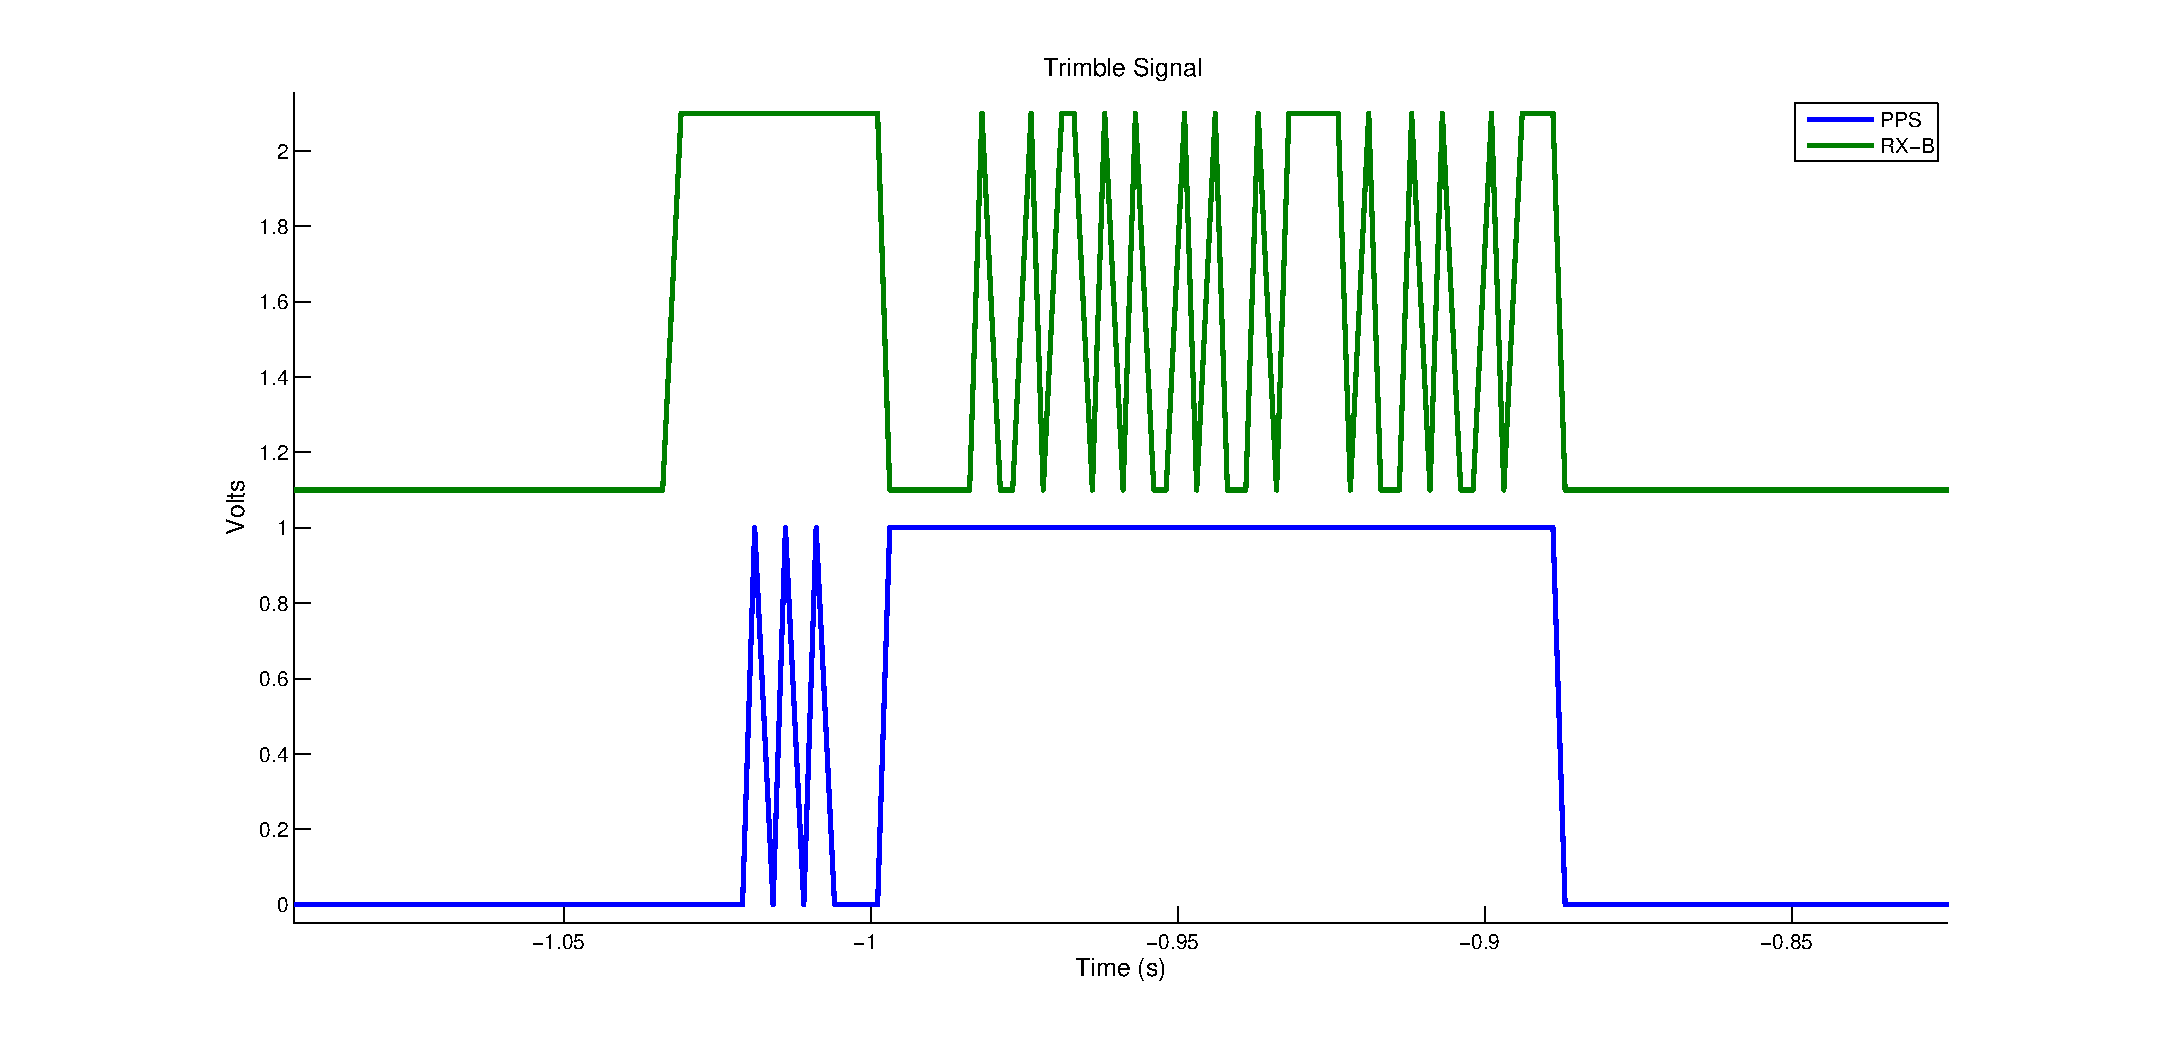
\includegraphics[width = 0.75\linewidth]{Trimble}
\caption{\textit{GPS sentence data and PPS signal recorded with oscilloscope for preliminary analysis.}}
\label{fig:GPS_PPS}
\end{figure}
%\end{landscape}
		\subsection{CORS}
		\subsection{Analog to Digital Converter}
			%\section{Analog-to-Digital Data Converter}
\subsubsection{Necessary Specifications}
\label{sec:ADC_Parameters}
\indent The BeagleBone Black microcontroller features an on board 12-bit analog-to-digital converter (ADC). From literature, the lowest acceptable
effective resolution that an ADC being used for SHM may have is 16 bits\cite{Cunha_Caetano} \cite{JangSWMWSS}. It was determined that the need for an
external ADC was present. The parameters of the external ADC needed were as follows:
\begin{itemize}
\item High Resolution
\item Appropriate Sampling Frequency
\item Low Power Consumption 
\item Support for Multiple Input Channels
\item Communicate via Serial Interface
\end{itemize}
\paragraph{Resolution}
\label{sec:adc_res}
\indent Resolution is defined as the number of bits that an analog signal is mapped to after being converted\cite{MusaJouaneh:2013}. Using the chart in
Figure \ref{fig:ADC_Comp_Chart}, it was evident that in order to achieve high resolution data that a Delta-Sigma ($\Delta\Sigma$) ADC needed to be used.\\
\indent As previously stated, the minimum resolution required for this sensor package was 16-bits. The voltage resolution can be found using Equation
\ref{eqn:Resolution}:
\begin{equation}
\label{eqn:Resolution}
V_{Res} = \frac{V_{Range}}{2^{n}}
\end{equation}
Assuming $V_{Range}=3.3V$, $n=16$ bits then $V_{Res}$ is approximately $50.35\mu V/$division. 

\begin{figure}[H]
\centering
\includegraphics[scale=1]{KIRBY_Images/ADC_Comp_Chart.jpg}
\caption{\textit{Chart displaying the classifications of different ADC architectures \cite{WaltKester:2005}}}
\label{fig:ADC_Comp_Chart}
\end{figure}
%
\paragraph{Sampling Rate}		%EDIT THIS SECTION
\label{sec:adc_fin}
\indent The Nyquist-Shannon Sampling Criterion states that data must be sampled at a minimum of twice the expected frequencies being measured
\cite{MusaJouaneh:2013}. The accelerometer that was chosen for the preliminary lab experiments has a bandwidth of $500 Hz$, therefore the ADC must be able
to sample a minimum of $1kHz$. However, since frequencies expected from the lab testing are in the range of $0-60Hz$, the sampling frequency of the ADC
does not necessarily need to be so high. %Must reference source that states expected natural frequencies of bridges
%
\paragraph{Power Consumption}
\label{sec:adc_power_cons.}
\indent Since the nature of this sensor package was to be a wireless sensor, it was assumed that all power used by the sensor package would be generated
using alternative energy. With this in mind, components used on board the sensor package have as little current draw as possible.
%
\paragraph{Input Channels}
\label{sec:adc_in_ch_num}
\indent One important, but almost overlooked, characteristic of the ADC was the ability to support multiple input channels simultaneously. The ADC needed
to be able to read three channels from an accelerometer and at least two channels from a strain gauge. For prototyping purposes, it is typically difficult
to find ADC's with more than 4 inputs; most come in as surface mount components and require a printed circuit board. It became evident as the project progressed that each input device would need a dedicated ADC due to the multiplexer switching time of multi-channel ADC units. 
It was decided to address this problem by interfacing four ADC units simultaneously on a serial communication bus.
Subsection \ref{sec:adc_comm} discusses this in further detail.
It should also be noted that the inputs of the ADC were configured for differential measurements.
This gives the ability to compare the sensor data to a noise reference, and thus make reducing data filtering during processing. 
%
\paragraph{Communication}
\label{sec:adc_comm}
\indent As shown in Table \ref{tab:uProcOptions}, the BeagleBone Black supports multiple communication protocols, include but not limited to, SPI and
I$^{2}$C. The communication from the ADC to the main micro-controller was decided to be either  4-wire SPI or I$^{2}$C. The ADC will be the slave to the
micro-controller. A con using SPI as the communication method is that for each slave device in the communication loop, there must be a dedicated Slave
Select (SS) line. This puts a limitation on how many ADC's can be used in each sensor package. However, I$^{2}$C utilizes a central bus and 7 bit unique
addresses for slave selection.

\subsubsection{Analog-to-Digital Converter Selection}
\indent When searching for ADC's that fit the parameters set in Section \ref{sec:ADC_Parameters}, three devices were investigated; the TI ADS1211, TI
ADS1115 and the TI ADS1113. The devices are summarized in Table \ref{tab:ADC_Compare} and explained in detail below.

\begin{table}[H]
\begin{center}
\begin{tabular}{|p{3cm}| p{3cm} | p{3cm} | p{3cm}|}
\hline
&\multicolumn{3}{c|}{\textbf{Analog-Digital Converter}}\\
\hline
\textbf{Parameter} & ADS1211 & ADS1115 & ADS1113\\
\hline
Package &\includegraphics[width = 2.5cm]{KIRBY_Images/oldadc}
&
\includegraphics[width = 2.5cm]{KIRBY_Images/ads1115} & \includegraphics[width = 2.5cm]{KIRBY_Images/ADS1113_msop10}\\
\hline
Resolution: & 24 bits & 16 bits & 16 bits\\
\hline
Supported Communications:&	 SPI & I$^2$C & I$^2$C \\
\hline
Power Consumption:&	5mW @ 5V	& 0.66 mW @ 3.3V & 0.66 mW @ 3.3V\\
\hline
Number of Inputs: & 4 & 4 & 1\\
\hline

\end{tabular}
\caption{\textit{Comparison table of the ADS1211, ADS1115 and ADS1113 ADC devices}}
\label{tab:ADC_Compare}
\end{center}
\end{table}


\paragraph{TI ADS1211}
\label{sec:ADC_ADS1211}
\indent The Texas Instruments ADS1211 24-Bit $\Delta \Sigma$ analog to digital converter features 20 effective bits of resolution at $1kHz$ under ideal
conditions; however that would be contingent upon the ability to design an ideal printed ciruit board (PCB) for the converter. Between 16 and 18 bits of
resolution are realistic for the initial prototype of the sensor package. By utilizing an internal 4-to-1 multiplexer, four input channels are available
to use. Recall that Section \ref{sec:adc_in_ch_num} requires at least five input channels, the ADS1211 falls short here. As a solution two ADC's would
be used, making it possible to read two strain gauges per sensor package as opposed to one. The ADS1211 datasheet provides information on synchronizing
multiple ADC's together. The converter draws approximately $10mA$ under typical working conditions. The converter utilizes the SPI protocol that is
supported by the BeagleBone Black.\\
\indent The ADS1211 was purchased and interfaced; however due to the complex circuitry that was required by the device, a month passed before the chip was
tested. The converter functioned correctly for approximately ten minutes and then stopped transmitting data. 
\paragraph{TI ADS1115}
\label{sec:ADC_ADS1115}
\indent The Texas Instruments ADS1115 16-Bit analog to digital converter is of the same architecture as the ADS1211 ($\Delta \Sigma$). The chip also
features a multiplexer that allows up to 4 single ended or 2 differential inputs. The sampling frequency of the ADC is programmable from 8Hz to 860Hz, and
includes an internal oscillator. The average current draw for the ADS1115 is approximately $150\mu A$. There are two notable differences between the
ADS1115 and the ADS1211 ADCs. First, the ADS1115 communicates via the I$^{2}$C communication protocol. The ADS1115 has four unique I$^{2}$C addresses;
making it possible to have 16 single-ended inputs on one communication bus. Also, the chip was available pre-mounted on a PCB with all the necessary
supporting hardware; thus eliminating the possibility of incorrectly wiring up the circuit. 
\paragraph{TI ADS1113}
\label{sec:ADC_ADS1113}
\indent The TI ADS1113 is within the same family as the ADS1115, only differing in the number of input channels and not having internal programmable gain amplifiers and comparator.
Like the ADS1115, four ADS1113 units can be on the same I$^{2}$C bus, can also run in continuous sampling mode, and also shares the same library of functions as the ADS1115.
Since the ADS1113 does not multiplex its inputs, there is no loss of data between switching.
The dissadvantage to the ADS1113 is that it is only available as a surface mount chip (MSOP-10 package); thus requiring more circuitry on the printed circuit board.

\paragraph{ADC Impedance Matching}
\label{sec:ADC_Impedance_Issues}
Preliminary lab tests were performed using a micro-controller with 12-bit ADC to collect data for analysis.
The time series that was returned did not accurately represent the data present, as verified with an oscilloscope.
It was determined that this was due to a difference in impedances between the accelerometer and the ADC.
The solution was to construct an op-amp circuit to match the impedances of the accelerometer and the micro-controller inputs.
It was initially believed that the internal programmable gain amplifiers (PGA) of the ADS1115 would avoid such issues in impedance matching.
However, after further research it was discovered that this assumption was incorrect.


\paragraph{ADC Final Selection}
\indent Based on the comparison of the ADS1211, ADS1115 and ADS1113 ADC's, the ADS1115 was chosen for the preliminary package to test code before the printed circuit board was designed.
For the final package, four ADS1113 ADC units were integrated into the PCB design as discussed in Section \ref{sec:ADC_Impedance_Matching}. 

	\section{Electrical Design}
			\subsection{Introduction}

\subsection{Circuitry}
For the 
\subsection{Printed Circuit Board}
	\section{Software Design}
		%\section{Software Design}
The software design controls the timing and data collection for the
package. The software structure is simple, yet crucial. In order to
keep the data collected by the package relevant, the software
logic and timing needed to be in order. \\

The first state in the software design is the initialization state.
Here, the analog to digital converter was initialized through I2C
communication. The handle of the analog to digital communication
object was saved for later use in the next state. Once the
initialization state was finished, the application proceeded
to the sampling state.\\

In this application, 200 Hz was decided to be the target sampling
rate. The program waited for an interrupt then the system time 
has reached a user-defined time. This is important because every 
sensor package waited for the same time and they sampled  
at the same instant (accurate to a millisecond). When the signal was received, 
the application proceeded to collect data from the peripheral sensors. For
each sample during the sampling duration, data was collected
from the ADC via I2C. The data structure was appended over the sampling entire
sampling period and passed as a return from the state.
Once the sampling duration was over, the data logging
state was begun. \\

The data logging state received the data structure created in the
previous sampling state. This data was then sorted and written to a
standard comma delimited text file. The file stream was closed
once all of the data had been written and the program finishes. A
simple block diagram of this flow can be seen in Figure
\ref{fig:PRO_SoftFlow}.

\begin{figure}[H]
\centering
\includegraphics[width = 4in]{"Software flow"}
\caption{\textit{Software flow of the sensor package}}
\label{fig:PRO_SoftFlow}
\end{figure}
	\section{Package Power}
		\subsection{Power Budget}
		\subsection{Energy Scavenging Potential}
			\subsubsection{Wind Potential}
			\subsubsection{Solar Potential}
		\subsection{Battery Selection}
		
\chapter{Data Collection}
\label{ch:DataCollection}
	\section{Phase One Data Collection}
		\subsection{6g Tri-Axial Accelerometer Data}
			\input{Paul_DataCollection_6gTri-AxialAccelerometerData}
	\section{Phase Two Data Collection}
		\subsection{6g Tri-Axial Accelerometer Data}
		\subsection{Cell Phone Accelerometer}
		\subsection{Battery Discharge Curve}
		\subsection{Experimental Observed Efficiency}
		
\chapter{Data Analysis}
\label{ch:DataAnalysis}
	\section{Phase One Data Analysis}
		\subsection{Comparison of Preliminary Abaqus Model and Preliminary Data}
			%\chapter{Data Analysis}
%
%\section{Phase One Data Analysis}
%
%\subsection{Comparison of Preliminary Abaqus Model and Preliminary Data }

\indent The results of the best experimental data for the 6g
 accelerometer on the angle beam are shown in Table
  \ref{tab:Results_Comp}.\\
\begin{table}
\begin{center}
    \begin{tabular}{|l| p{3.5cm}| p{3cm}| p{3cm}| p{3cm}|}
    \hline
    \textbf{Mode} & \textbf{Analytical Values} & \textbf{Values for the generalized profile} & \textbf{Values for the Input profile} & \textbf{Experimental} \\\hline
    1    & 3.1 Hz            & 3.1 Hz                             & 3.1 Hz                       & 3.2 Hz       \\\hline
    2    & 12.4 Hz           & 12.5 Hz                            & 12.4 Hz                      & 12.5 Hz      \\\hline
    3    & 27.9 Hz           & 27.8 Hz                            & 27.8 Hz                      & 27.6 Hz      \\\hline
    4    & 49.6 Hz           & 48.8 Hz                            & 48.6 Hz                      & 48.4 Hz      \\\hline
    5    & 77.5 Hz           & 74.5 Hz                            &                             & 78.5 Hz      \\\hline
    \end{tabular}
    \caption{\textit{Comparison between analytical, model and experimental results}}
    \label{tab:Results_Comp}
\end{center}
\end{table}
\begin{table}
\begin{center}
    \begin{tabular}{|l|l|l|l|}
    \hline
    Mode & Analytical Frequencies [Hz] & Experimental Frequencies [Hz] & Percent Difference \\
    \hline
    1    & 3.1                         & 3.2                           & 3.1                \\
    2    & 12.4                        & 12.5                          & 0.80               \\
    3    & 27.9                        & 27.6                          & 1.1                \\
    4    & 49.6                        & 48.4                          & 2.5                \\
    5    & 77.5                        & 78.5                          & 1.3                \\
    \hline
    \end{tabular}
    \caption{\textit{Comparison between analytical and experimental results}}
    \label{tab:ExperimentalvsAnalytical}
\end{center}
\end{table}
A direct comparison between the experimental values and the frequencies may be found in Table \ref{tab:ExperimentalvsAnalytical}.
As the experimental data and the analytical values are very similar the 6g accelerometer can be considered to be taking viable, accurate data.
The first test was done using a piezoelectric strip to detect vibration. The second series of tests was done with a 3g accelerometer (anything above acceleration of 3g is clipped). The third series was done with a 6g accelerometer.

	\section{Phase Two Data Analysis}
		\subsection{Comparison of Developed Abaqus Model with Literature}
			\subsection{Phase Two Data Analysis}

\subsubsection{Comparision of Developed Abaqus Model with Liturature}


In verifying the results of the model produced in Abaqus experimentl data taken on the Claiborn Pell Bridge that were published in the Journal of the
Structural Division. Upon completion in 1969 a study involving seven seismometers estimated the first 20 modes, 11 normal modal response shapes, and 20
critical damping locations. Traffic, wind, and other environmental factors loading was measured by seismometers. The direct power spectral density by
way of the Ambient Vibrations Survey method was found of each recorded motion, estimates of the natural frequencies were produced. An Ambient Vibration
Survey (ASV) was performed on the bridge on August 20-22, 1969. During experimentation, approximately 8,000 vehicles passed over the bridge each day
and winds were moderate. Seven seismometers were arranges in five different orientations to properly capture the modal shapes. 20 natural
frequencies, 11 normal mode shapes, and 20 critical damping estimates are presented. The First 20 modes of vibration ranged from 0.155-0.993 Hz,
modal shapes for the first 5 symmetric vertical modes can be seen in \ref{fig:Paul_Modes1-5}\\

\begin{figure}

\centering

\includegraphics[width=\linewidth]{Paul_Modes1-5}

\caption{The modal responce for the first five modes of the Caliborn Pell Bridge.}

\label{fig:Paul_Modes1-5}

\end{figure}

In table \ref{tab:

the first five modal frequencies produced by the Abaqus model and that indicated by the Journal atricle.  


\begin{table}
\begin{tabular}{lllll}
Mode & Abaqus Model Frequencies [Hz] & Journal Article Frequencies [Hz] & Percent Difference \\
1    & 0.16                          & 111                              & \%11               \\
2    & 0.42                          & 222                              & \%22               \\
3    & 0.52                          & 333                              & \%33               \\
4    & 0.64                          & 444                              & \%44               \\
5    & 0.71                          & 555                              & \%55               \\
\end{tabular}
\caption{First five modes comparision for Abaqus and Journal Article}
\end{table}

		\subsection{Comparison of Developed Abaqus Model with Developed Abaqus Model}	
		
\chapter{Future Development}
\label{ch:FutureDevelopment}
	\section{Instrumentation}
		\subsection{Integration of Strain Gauge}
			\subsubsection{Integration of Strain Gauge}

\indent Figure \ref{fig:OmegaSoldered} is one of the 3-element rosette strain gauges with pre-soldered ribbon leads. Purchased from omega engineering with
model number SGD-6/120RYT23. These strain gauges were necessary after realizing the difficulty of soldering leads to the original set of strain gauges. The
pre-soldered ribbon leads on the second set of strain gauges also proved to be unsuccessful during experimentation. This was because the leads would not
stay secured to the attaching clips while tests were being run. Even with the persistent attempts to get the strain gauges connected and working
correctly, the data received was still very inaccurate. One possible contributing factor to this may have be the lack of precision when applying the
strain gauge to the exact location on the beam. However, one definite factor that contributed to the inaccurate data from the strain gauges was the
type of strain gauge that was used. A strain gauge with a different gauge factor and a higher resistance would have been more favorable. The higher
the resistance of a strain gauge, the higher the sensitivity. The original sets of strain gauges had a resistance of 120 $\Omega$, but to precisely
measure strain on a beam the resistance must be much higher, 350 $\Omega$ or more. The costs for a pack of 6 similar strain gauges with a resistance of
350 $\Omega$ from omega engineering is one hundred dollars. Another factor that halted the efforts to apply the strain gauge was that they required
another ADC output. It is possible to make more outputs, however this also demands that the time synchronization is even more accurate.
Nevertheless, higher resistant strain gauges would be better for sensor packages for future developments. \\

\begin{figure}[h]
\centering
\includegraphics[width=0.3\textwidth]{Strain_Gauge_with_Leads.png}
\caption{\textit{Omega 3-Element Rosette with pre-soldered leads.}}
\label{fig:OmegaSoldered}
\end{figure}
		\subsection{Wireless Transmission}
			\label{sec:XBeeFuture}
		\subsection{GPS Time Synchronization}
		\subsection{Package Assembly}
			\subsubsection{Fabrication of Circuit Board}
			\subsubsection{Battery Integration}
			\subsubsection{Power Management}
			\subsubsection{Package Enclosure}
				\section{Package Enclosure}

When the components are tested and fully operational in laboratory conditions, they will need to be packaged into the casing. The following
characteristics need to be considered when determining which case is best suited for this application:

\begin{itemize}
\item {Quality} 
\item {Size/Orientation}
\item {Heat Dissipation} 
\item {Cost} 
\item {External Connectors}
\end{itemize}


When the package is mounted onto the Newport Bridge, it will be exposed to harsh weather conditions: wind, precipitation, extreme temperatures,
etc. Therefore, it is essential to utilize a case that can withstand these conditions. O-rings are necessary to prevent water from leaking into
the case through the seal of the lid. This water can easily damage the electrical components within the package. The case will also have to be able to
withstand possible extreme temperatures. If the case cannot withstand the possible cold temperatures it will be exposed to without cracking, water can
leak into the package and destroy the equipment. High temperatures can cause the case to melt/deform which may possibly affect the retrieved data. 

It will be important to choose a case that not only large enough that can house all of the equipment but also fits the equipment in a manner that it can
be neatly organized and arranged. This allows for a quicker and more efficient package assembly. This also allows for a quicker examination of the
set-up in case an error occurs. To account for this, the orientation of the case is important. For example, a top-loading bucket (such as the Pelican
1430 seen below) would not be practical because it would be very difficult to access the components once the package is assembled and mounted.  



Electrical devices are only operational within a specific temperature range where if the maximum or minimum temperatures are exceeded, the component may
not fully function or even fail completely. To determine if the SHM system will fail due to extreme temperatures, the temperature inside the case must
be calculated. The enclosed volume has two major sources of temperature flux: the external temperature and the work done by the system. The first step
will be to calculate the heat transferred from the electrical components using the equation:

\begin{equation}
q(eq) = P(eq)*K_1*K_2
\end{equation}

where $q(eq)$ is the heat transferred from electrical equipment in Watts (W), $P(eq)$ is the electrical power consumption (W), $K_1$ is the load
coefficient, and $K_2$ is the running time coefficient. This value will then be inserted into the 1-D heat transfer equation:

\begin{equation}
q=k*A*\frac{\Delta T}{dx}
\end{equation}

where $q$ is the heat due to the electrical components, $k$ is the thermal conductivity of the material, $A$ is the area of which heat is being transfered
through, $\Delta T$ is the change in temperature, and $dx$ is the thickness of material. This equation will need to be computed for the heat transfer
through each of the casing walls, as well as the corners of the case, then averaged using the equation: 

$$q_t = sqrt((q_x)^2+(q_y)^2+(q_z)^2+(q_c)^2)$$

where $q_c$ is the heat transfer through the corners of the case. The resulting value will then be used with the maximum expected temperatures based on
temperature history data, such as that provided by NOAA, to determine the maximum temperature at which the system will still operate. If the resulting
temperature is higher than the lowest maximum operating temperature out of all the components, the system may fail, and that case may not be the best
option. That same principal can be applied to when the system is not generating any heat with respect to the minimum expected external temperature and
highest minimum operational temperature of the components. Ideally, once the package is fully modeled, the heat transfer equation can be more
thoroughly and accurately calculated by accounting for the spatial orientation between the components and the interior walls of the case. However,
if the components are mounted in place via foam cutouts, the heat dissipation between the components and the foam must first be calculated, and then
the heat transfer between the foam and the interior walls will then be calculated.

\paragraph{External Connectors} 
Several external connectors will need to be installed on the case walls for the full functionality of the SHM system. These ports need to be waterproof
with tight seals to prevent water from entering the case or external connections. The waterproof connections will require secure mating mechanisms, such
as locking and screwing mechanisms shown in Figure \ref{fig:BowChicaWowWow}, to ensure that that the male ends will not become unplugged thus allowing
water to enter the connection and damage it. Each connector will also require a bulkhead cap to cover and protect against water damage if the
connector is not in use. These external connections are going to be implemented for a variety of sub-systems within the SHM package: energy
scavenging devices, BeagleBone Black, strain gauge, GPS, and XBee.
\begin{figure}[h]
\centering
\includegraphics[width=0.3\textwidth]{Wiley_MatingStyle.JPG}
\caption{\textit{Example Mating Mechanisms}}
\label{fig:BowChicaWowWow}
\end{figure}

Power connectors will be used to connect the wind turbine and solar panels to the package. These connectors must be rated for a high enough current to
match the power source. For example, since the wind turbine is rated up to 27A, the power connector should have a current rating that is similar enough
that there will not be damage done to the port due to the excess current. Each power connection will have a female port installed on the side of the
case and a corresponding male jack will need to be installed at the end of the power input. If multiple solar panels are utilized, either the power
inputs need to be put into parallel in one wire to input all the energy through one connection or a connector needs to be installed for as many panels
are used. 

A USB 2.0A port will be installed to access the BBB without having to open the package via a flash drive. This type of USB port was chosen to match the
same type of connection specified from the BBB data sheet. The connector gender of this port needs to be female to plug a USB chord to access the BBB,
such as the one seen in Figure \ref{fig:USB}. 
\begin{figure}[h]
\centering
\includegraphics[width=0.3\textwidth]{Wiley_USB2Aport.JPG}
\caption{\textit{USB 2.0A External Connector (LTWUA-20AMFM-SL7A) from Ampehnol LTW}}
\label{fig:USB}
\end{figure}

There are a few different types of connectors that can be used to attach the leads of the strain gauge to the package. Unlike the rest of the
connections, the strain gauge leads do not require a certain type of connection terminal. One option is to attach the leads to either a category 5 (CAT
5) or CAT5e shielded Ethernet cable and install an external connection for such a cable as seen in Figure \ref{fig:CAT5}. Category type cables are
designed for high signal integrity to achieve performance standards set by organizations \cite{gareis2003surfaced}. This type of cable will ensure that the signals are relayed to the ADC reliably. A shielded cable is desired to
ensure that the sensitive signal being sent from the strain gauge to the ADC does not get disturbed by noise. 
\begin{figure}[h]
\centering
\includegraphics[width=0.3\textwidth]{Wiley_CAT5EthernetConnection.JPG}
\caption{\textit{Shielded Ethernet External Connector (RJ45-5EWTP-QR-PCB) from Video Production Inc}}
\label{fig:CAT5}
\end{figure}

An alternative method is through the use of waterproof cable glands (see Figure \ref{fig:Cable Gland}. The leads would be attached to a cable, preferably
shielded, and fed through the gland which would then be sealed. The proper gland must be matched up to the outer diameter of the cable otherwise the
gland will not be water tight. These are advantageous because not only do individual cable glands work with a range of cable thicknesses, but different
gland diameter ranges can be found. 
\begin{figure}[ht]
\centering
\includegraphics[width=0.7\textwidth]{Wiley_CableGland.JPG}
\caption{\textit{Cable Gland (CB-GD-5000045) from AA Power Corp}}
\label{fig:Cable Gland}
\end{figure}


The GPS antenna attaches to the GPS via the use of a coaxial MCX connection. Two viable options for connecting the antenna are to implement a waterproof
MCX connector or a cable gland. Implementing a waterproof MCX connector on the package may be difficult because MCX connectors are very small as evident
by Figure \ref{fig:MCX}. If one of these connectors is able to implemented, it will be essential to choose the proper impedance level of the
connector. The other option is to implement a cable gland, such as the alternative option for the strain gauge above in Figure \ref{fig:Cable Gland},
to run a wire through the case wall between the antenna and the GPS. The antenna would then need to be fastened to the outside of the case or another
substrate to prevent it from freely swinging around. 
\begin{figure}[ht]
\centering
\includegraphics[width=0.7\textwidth]{Wiley_MCX.JPG}
\caption{\textit{MCX Jack-to-Jack Adapter (252171) from Aamphenol Connex with Size Reference}}
\label{fig:MCX}
\end{figure}


The final component that requires and external connector is the XBee.The XBee antenna attaches to the device itself via the use of an SMA connection. A
waterproof coaxial connector, like the one shown in Figure \ref{fig:SMA}, can be implemented as the external connector as well as a cable gland. 
Similarly to the MCX connector, the SMA connector is also small which may make utilizing one of these difficult. However, if a cable gland is used, the
antenna may need to be mounted to the case or other substrate to prevent it from freely swinging around as is the case with the GPS.
\begin{figure}[ht]
\centering
\includegraphics[width=0.7\textwidth]{Wiley_SMAconnector.JPG}
\caption{\textit{Waterproof SMA Bulkhead Connector (9153-7553-002) from Applied Engineering Products with Size Reference}}
\label{fig:SMA} 
\end{figure}



\paragraph {Case Selection} Attempts were made to try to obtain the actual thermal conductivity coefficients for different cases, but unfortunately proper
data was never able to be retrieved due to lack of information from retailers. Since the general material of the considered cases is known, an
estimation of the thermal conductivity coefficient was made because studies have been performed to determine $k$ values for different materials. 
However, continued efforts to obtain this information may supply data to more accurately calculate the heat transfer through the casing walls. The
thickness of each case will need to be considered for two reasons. The first reason is that the thickness of the case affects heat transfer. Thicker
cases will allow for less heat transfer through the casing walls. The other is that the thickness of the casing wall affects whether or not certain
external connectors can be implemented. If the case is too thick, many MCX and SMA connectors may not be able to be installed because the case may
be thicker than the connector is long. When comparing costs, it should be later noted of any accessories, whether they are necessary or
convenient, that can and will be purchased. For example, the Ultra-case 613 by UW Kinetics charges another \$6.99 for the required O-ring to
water proof an already expensive case, so this may not be the most suitable case for this application. For a look at the a comparison of nominal
characteristics of the cases that were considered, see \ref{sec:Appendix Case Comparison}.

\paragraph{Assembly Layout}
When the package is ready to be assembled, the interior layout of the components needs to be determined. A few factors will need to be considered. 
The first is the location of external connectors. As stated above, the thickness of the case will affect what type of connectors may need to used. 
An example of this is shown in Figure \ref{fig:Assembly} which is a potential 2-D assembly layout using a Pelican 1400 model case. If an SMA
connector is used instead of a cable gland, it would need to be installed on the shorter wall since the case does not have a uniform thickness and
that wall is the only one thin enough out of the two to install such a connector. It would not make to sense to install the connectors through
the lid either because opening the case may place too much tension on the wires causing damage. 

\begin{figure}[h]
\centering
\includegraphics[width=1\textwidth]{Wiley_2DAssemblyLayout.jpg}
\caption{\textit{Potential Layout of a Pelican 1400 Model Case.
The red arrows depict a 12V power supply, the yellow arrows depict a 3.3V power supply, and the green arrows depict the transfer of communications.}}
\label{fig:Assembly}
\end{figure}

It will also be important to orient the breadboard in a manner that the accelerometer measures data in the intended direction as if it was mounted. 
Otherwise, it will need to be understood that the data measured on each axis during lab trials will not be measured along the same axes in the field and
will need to be accounted for while analyzing the data. 

			\subsubsection{Package Location}
				\section{Package Location}

\indent Figure \ref{fig:PackageLocation} is an Abaqus visualization of the Newport Bridge with the proposed location for the sensor package to be mounted.
As shown in the figure, the center of the bridge is the best location for the sensor package. This is because the greatest amplitude of displacement will
occur during the first mode of vibration at the middle of the bridge. Mounting the sensor package to the bridge must be done without damaging the
structure in any way. The sensor package must also be capable of being moved easily. Most importantly, the package must be secured without any of its
own motion so that the sensors can recognize the movement of the bridge and not the movement of the package itself. 

The most economical way of securing the sensor package to the bridge is to use powerful magnets. Neodymium Magnets are strong magnets that work well in
all environments and resist demagnetization. One negative aspect of magnets is that they can be prone to corrosion if a protective coating is not
properly applied. There is also a concern that the magnetic field can disrupt the electronics within the case. However, these issues can be prevented if
the correct precautions are taken. These magnets come in many shapes and sizes, as shown in Figure \ref{fig:Mounting Magnet}, and can be purchased with
pre-fabricated holes for screws to attach the magnets to the exterior of the case. The magnets in figure \ref{fig:Mounting Magnet} are the MMR-A-XC
model of magnets from KJMagnetics.com. This magnet is hardly larger than a penny, yet it can easily be screwed into the sensor package and has a
holding force of 54.14 pounds. With two of these magnets screwed into the case, the package would be secured to the bridge. If data analysis is
performed to prove the wind speed on the surface of the package to be too much for this pull force, stronger magnets are available. KJMagnetics.com
also has similar magnets but with different pull forces ranging from 26.8 pounds to 260 pounds. These magnets can be used for securing the solar
panels and wind turbine as well. 

\begin{figure}[ht]
\centering
\includegraphics[width=0.3\textwidth]{Neodymium_Mounting_Magnet.jpg}
\caption{Neodymium Mounting Magnet.}
\label{fig:Mounting Magnet}
\end{figure}

Figure \ref{fig:Proposed Package, Panels and Turbine Location} shows a practicable location for the sensor package along with the solar panels above and
the wind turbine hanging just below. The sensor package should be mounted on the outside of one of the major vertical beams at midspan of the bridge. The
solar panels and wind turbine must be mounted close within a reasonable distance to keep the cable length to a minimum. The best place to mount the
solar panels is on top of the upper horizontal beam on the southern side of the bridge. This will allow for the most amount of sun light and the
shortest amount of cable necessary. The best place to mount the wind turbine is on the bottom of the lower horizontal beam on the southern side of the
bridge. This location has plenty of wind because it is above the middle of the Narragansett Bay. By mounting the sensor package, solar panels and
wind turbine below the deck on the southern side of the bridge the package will be capable of producing its own power and accurately measuring the
vibrations of the bridge.


\begin{figure}[ht]
\centering
\includegraphics[width=0.3\textwidth]{Bridge_Full_.png}
\caption{Proposed Package Mounting Location.}
\label{fig:PackageLocation}
\end{figure}


\begin{figure}[ht]
\centering
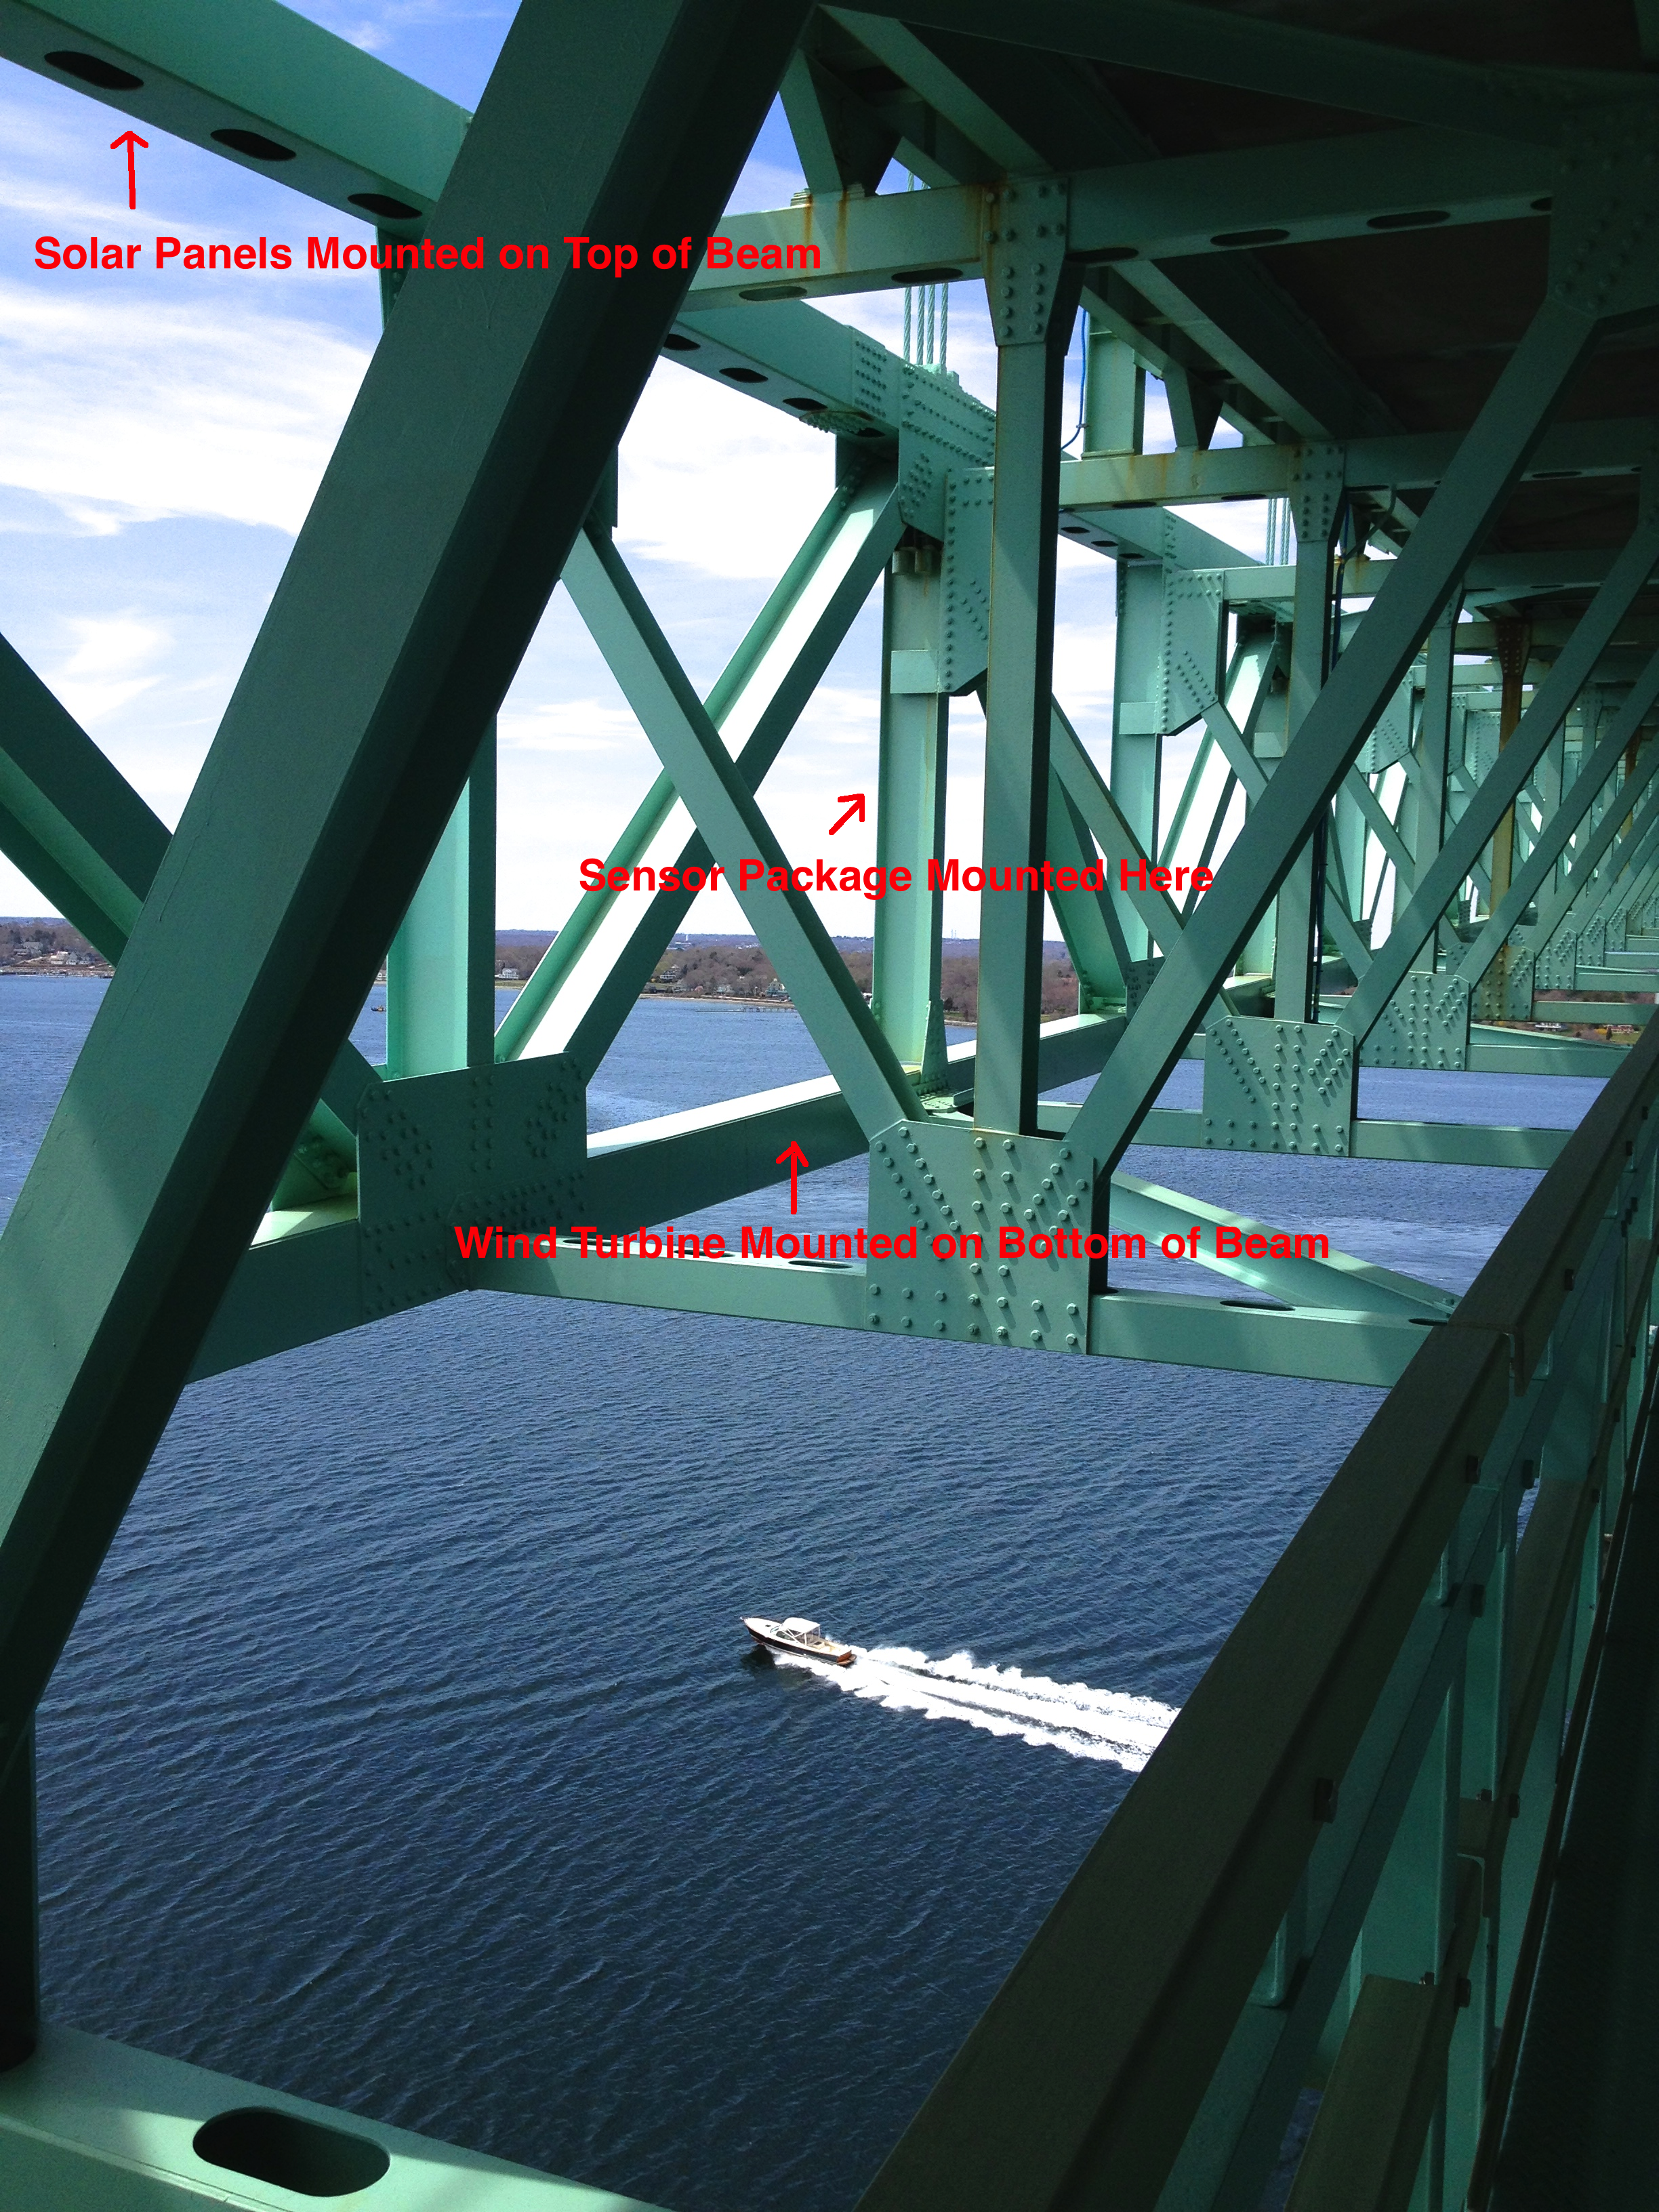
\includegraphics[width=0.3\textwidth]{Proposed_Package_Location.png}
\caption{Proposed Location for Sensor Package, Wind Turbine and Solar Panels.}
\label{fig:Proposed Package, Panels and Turbine Location}
\end{figure}

	\section{FEM}
		%\section {Finite Element Model}

\subsection{Model Improvements}

The Abaqus model produced for this project can be further developed to produce more accurate modal responses to static and dynamic loading. Any improvement to the model will replicate the bridge more closely. The longterm effect of fatigue is immeasurable and will create an unavoidable error. After measuring the current natural frequency of a bridge an original stiffness matrix can be estimated from the bridge a stiffness matrix can be estimated and inputed to Abaqus, however, evaluation the effects of fatigue on structural integrity is difficult.    
\indent The current model is considered to be one cohesive piece with a uniform stiffness rather than different individual sections that are bolted or welded together. In a more precise model, as the 19,0000 element model produced for evaluating the Tsing Ma Bridge in Hong Kong, each piece of the bridge was modeled to reflect the actual material. The steel cables were molded as thousands of steel wires and the road deck was modeled as pavement \cite{Chan}. As steel is primarily used for the entire structure of the Claiborn Bridge the error acquired is relatively small. 
\indent Suspension bridges will deform plastically everywhere accept for the welded regions which should be modeled as rigid pieces. These joints are critical locations in the system as fatigue cracks will develop first. If the welds that are under the most stress can be identified they can be reinforced or monitored more closely \cite{Chan}. Bridge scions that connect at bolts rather than welds have friction at the interface of the two sections. This friction is important when evaluating failure.

\subsection{Dynamic Loading} 

\indent In this evaluation, only static loading was evaluated as dynamic loading is outside the scope of this project. The model of the Tsing Ma Bridge was evaluated for dynamic loading as two mediums of traffic utilize this bridge. The trains and trucks that travel over the bridge require entirely separate analysis as they present the bridge with entirely different loading signatures.\\
\indent The loading of a train, individual truck in both lanes, and groups of trucks with varying orientation were simulated passing over the bridge. As a single truck will not affect the net dynamic response only the local response must be examined. To minimize computation time only relevant elements were applied a tapering load for less than 2 s and then eliminated from the simulation. Groups of trucks were separated by a 3 s lag time. The variability of traffic was examined and the co-existence of the two types of loading were quantified. A stress cycle was produced for each traffic variation and compiled to identify which element would experience the most intense local stresses. The critical locations of local stress under truck loading are the utmost part of the upper chord and the bottom cross-frame between the rail tracks. Under train loading the critical locations in the deck unit are at the utmost parts of the upper chord and show more stress than the highest local stress under truck loading. Because of this it was determined that an outbound train will produce the most stress in the upper chords along the bridge longitudinal direction. This location was chosen to determine fatigue critical locations in the whole bridge \cite{Chan}. 

		
\chapter{Conclusion}
\label{ch:Collection}
	
\chapter{Conclusions}
\indent Over the course of this two phase project a prototype of the sensor package was designed and partially assembled. A finite element model was produced and verified for the Claiborn Pell Bridge.  Development must be done on wireless transmission of data, time-synchronization of data and energy scavenging. It is anticipated that the final sensor package will have a custom PCB designed and fabricated to localize the microprocessor, ADC, accelerometer and GPS to one board.\\
\indent 



\bibliographystyle{plain}
\bibliography{./BIB_Files/WILEY_BIB,./BIB_Files/KIRBY_BIB,./BIB_Files/PAUL_BIB,./BIB_Files/IANNUCCI_BIB}

\appendix

\chapter{Sensor Package Schematics}
\label{app:Schematic}
\section{LM317 Adjustable Voltage Regulators}
\begin{figure}[H]
\centering
\includegraphics[width=\textwidth,height=\textheight,keepaspectratio]{Multisim_VoltageRegulation}
\caption{Schematic of 5V and 3.3V voltage regulator circuit}
\label{fig:Schematic_VoltageReg}
\end{figure}

\section{BeagleBone Black}
\begin{figure}[H]
\centering
\includegraphics[width=0.9\textwidth,height=0.9\textheight,keepaspectratio]{Multisim_BBB}
\caption{Schematic of BeagleBone Black}
\label{fig:Schematic_BBB}
\end{figure}

\section{MMA7361 Accelerometer}
\begin{figure}[H]
\centering
\includegraphics[width=\textwidth,height=\textheight,keepaspectratio]{Multisim_MMA7361}
\caption{Schematic of MMA7361 $\pm 1.5g/ \pm 6g$ Tri-Axial Accelerometer}
\label{fig:Schematic_MMA7361}
\end{figure}

\section{MCP606 Op-Amp Buffer Circuit}
\begin{figure}[H]
\centering
\includegraphics[width=\textwidth,height=\textheight,keepaspectratio]{Multisim_4OpAmp}
\caption{Schematic of MCP606 ADC Input Buffer Circuit}
\label{fig:Schematic_MCP606}
\end{figure}

\section{ADS1113 Analog-Digital Converter}
\begin{figure}[H]
\centering
\includegraphics[width=0.9\textwidth,height=0.9\textheight,keepaspectratio]{Multisim_4ADC}
\caption{Schematic of four ADS1113 ADC units in parallel}
\label{fig:Schematic_ADS1113}
\end{figure}

\section{Trimble Copernicus II GPS Receiver}
\begin{figure}[H]
\centering
\includegraphics[width=\textwidth,height=\textheight,keepaspectratio]{Multisim_GPS}
\caption{Schematic of Copernicus II GPS Receiver}
\label{fig:Schematic_Copernicus}
\end{figure}

\chapter{Enclosure Options}
\label{app:CaseOptions}
\begin{landscape}

\begin{table}[c]
\centering
\begin{tabular}{|c|l*{5}{|c}|p{2.5cm}|}
\hline
\multicolumn{8}{|c|}{\textbf{Enclosure Options}}\\
\hline
Company   & Case Model   & Length & Width & Height & Weight & Cost   & Thermal Conductivity Coefficient (W/m*$^{\circ}$C) \\
\hline
Pelican   & 1300      & 9.17  & 7.00 & 6.12  & 3.09  & \$55.65 & 0.1-0.22                       \\
~      & 1400      & 11.81 & 8.87 & 5.18  & 3.97  & \$81.58 & 0.1-0.22                       \\
~      & 1450      & 14.62 & 10.18 & 6   & 5.51  & \$103.73 & 0.1-0.22                       \\
~      & 1460      & 18.54 & 9.92 & 10.92 & 8.75  & \$180.59 & 0.1-0.22                       \\
Fibox    & PC MH 125 G  & 9.1  & 5.5  & 4.9  & NA   & NA    & 0.19                         \\
~      & PC 2828 18 G  & 10.9  & 10.9 & 7.1  & NA   & NA    & 0.19                         \\
~      & PC 175/150 XHG & 7.1  & 7.1  & 5.9  & NA   & NA    & 0.19                         \\
Nanuk    & 9.4      & 9.4  & 7.4  & 5.5  & 3.3  & \$38.95 & 0.1-0.22                       \\
~      & 915      & 13.8  & 9.3  & 6.2  & 4.4  & \$63.95 & 0.1-0.22                       \\
UW Kinetics & Ultra-case 613 & 13.4  & 8.9  & 5.6  & 4.5  & \$148.99 & 0.2                         \\
\hline
\end{tabular}
\caption{Brief summary of enclosure options considered for the sensor package}
\end{table}
\end{landscape}

\chapter{Battery Log}
\label{app:batterylog}
\section{Battery Log}
\label{app:BatteryLog}
\begin{table}[h]
\centering
\begin{tabular}{lllp{2.5cm}}
Filename   & 20140421T162625                &          &                                                                               \\
Battery    & 1-3                            &          &                                                                               \\
V initial  & 13.21 V                        &          & Test on new battery 1-3 with car light                                        \\
load       & Sylvania 3157                  &          &                                                                               \\
           & 26.88 W                        & 4.24 $\Omega$   &                                                                               \\
           & 12V                            &          &                                                                               \\
           & 2.1 A                          &          &                                                                               \\
           &                                &          &                                                                               \\
cut out    & 9 V                            & 10:19:39 &                                                                               \\
V open cir & 10.881 V                       &          &                                                                               \\
           &                                &          &                                                                               \\
\hline
Filename   & 20140422T113901                &          &                                                                               \\
Battery    & 1-3                            &          &                                                                               \\
V open cir & 10.881 V                       &          & Log  of open circuit voltage from previous test                               \\
           &                                &          &                                                                               \\
Filename   & 20140422T133734                &          &                                                                               \\
Battery    & 1-3                            &          &                                                                               \\
V initial  &                                &          & After fully discharged battery had rested for 2 hours it was discharged again \\
load       & Sylvania 3157                  & 4.24 $\Omega$   &                                                                               \\
           & 26.88 W                        &          &                                                                               \\
           & 12V                            &          &                                                                               \\
           & 2.1 A                          &          &                                                                               \\
cut out    & 9 V                            &          &                                                                               \\
V open cir & 10.881 V                       &          &                                                                               \\
           &                                &          &                                                                               \\
\hline
Filename   & 20140422T141819                &          &                                                                               \\
Battery    & 3-1                            &          &                                                                               \\
V initial  & 13.20 V                        &          & Part 1 of initial test on battery 3-1                                         \\
load       & 2 x 100Ω resistors in parallel &          &                                                                               \\
           & 49.648 Ω observed              &          &                                                                               \\
           &                                &          &                                                                               \\
\hline
Filename   & 20140423T104026                &          &                                                                               \\
Battery    & 3-1                            &          &                                                                               \\
V initial  & 13.20 V                        &          & Part 2 of initial test on battery 3-1                                         \\
load       & 2 x 100$\Omega$ resistors in parallel &          &                                                                               \\
           & 49.648 $\Omega$ observed              &          &                                                                               \\
cut out    & 8.962 V                        & 20:22:12 &                                                                               \\
V open cir & 10.96 V                        &          &                                                                              
\end{tabular}
\caption{Captions!~}
\end{table}
 

\end{document}
